% !TeX root = ../main.tex
\chapter{Numerical investigation}
\label{chapt:results}


\section{The fermionic correlator}
To start with the study of the model, we want to analyse the behaviour of the fermionic correlator and illustrate the fermionic masses extraction procedure. \\
Let us initially restrict to $g = 0$, so that \textcolor{red}{add wilson}
\begin{equation*}
    D_{n m}=\sum_{\hat\mu}\left[\frac{\gamma_{\hat\mu}\delta_{n+\hat\mu, m} - \gamma_{\hat\mu} \delta_{n-\hat\mu, m}}{2} + m_q \, \delta_{n m}\right] .
\end{equation*}
In this case, an analytical expression of the fermionic mass can be derived as follows. \\
The Dirac operator in momentum space reads
\begin{equation*}
\bar{D}(p)= m_q + \sum_\mu 2 \sin ^2\left(\frac{p_\mu}{2}\right)+i \sum_\mu \gamma_\mu \sin \left(p_\mu\right)
\end{equation*}
The inverse can be checked to be 
\begin{equation*}
    \bar{D}^{-1}(p) = \frac{m_q + \sum_\mu 2 \sin ^2\left(\frac{p_\mu}{2}\right) - i \sum_\mu \gamma_\mu \sin \left(p_\mu\right)}{\left[m_q + \sum_\mu 2 \sin ^2\left(\frac{p_\mu}{2}\right)\right]^2 + \left[\sum_\mu \gamma_\mu \sin \left(p_\mu\right)\right]^2}
\end{equation*}
One can now find the pole mass by imposing 
\begin{equation*}
    \left[m_q + \sum_\mu 2 \sin ^2\left(\frac{p_\mu}{2}\right)\right]^2_{p_\mu = (im_\text{phys}, 0)} + \left[\sum_\mu \gamma_\mu \sin \left(p_\mu\right)\right]^2_{p_\mu = (im_\text{phys}, 0)} = 0
\end{equation*}
This results in a trascendental equation 
\begin{equation*}
    \left[m_q - 2 \sinh^2\left(\frac{m_\text{phys}}{2}\right)\right]^2 - \sinh^2\left(m_\text{phys}\right) = 0
\end{equation*}
This equation has the solution 
\begin{equation*}
    m_\text{phys} = \log\left(1+m_q\right)
\end{equation*}
We then compute the correlator numerically via a single inversion of the Dirac operator as detailed in Appendix \ref{chap:AppendixC}. The lattice volume is chosen to be $128 \times 128$. 
\begin{figure}
    \centering 
    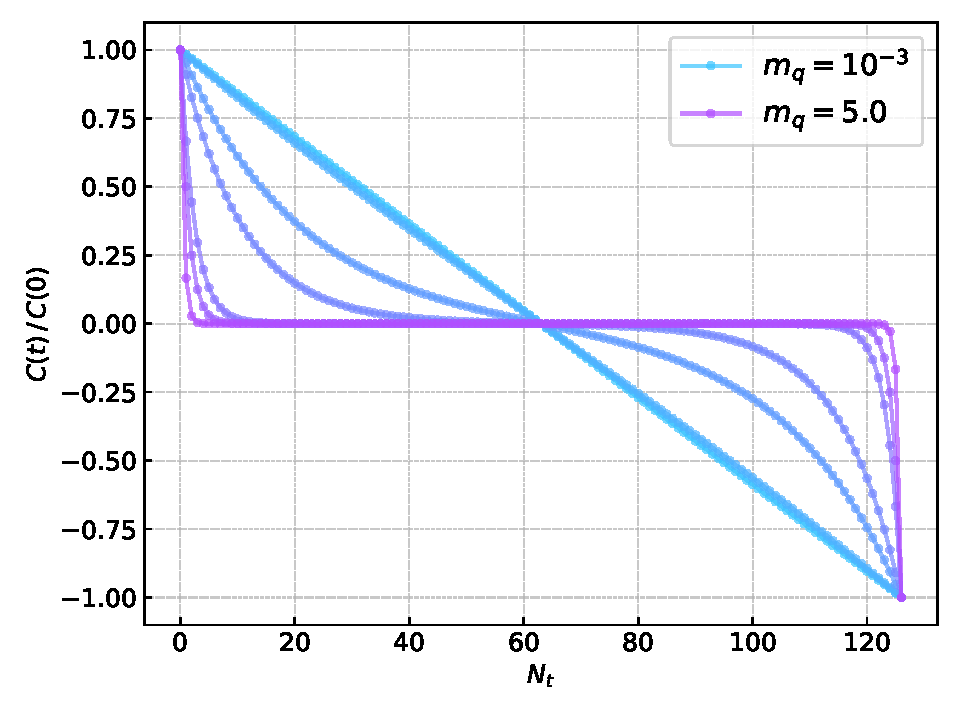
\includegraphics[scale=0.6]{figures/correlator/correlator.pdf}
    \caption{Correlator as a function of the bare mass}
    \label{fig:correlator_mass}
\end{figure}
\begin{figure}
    \centering 
    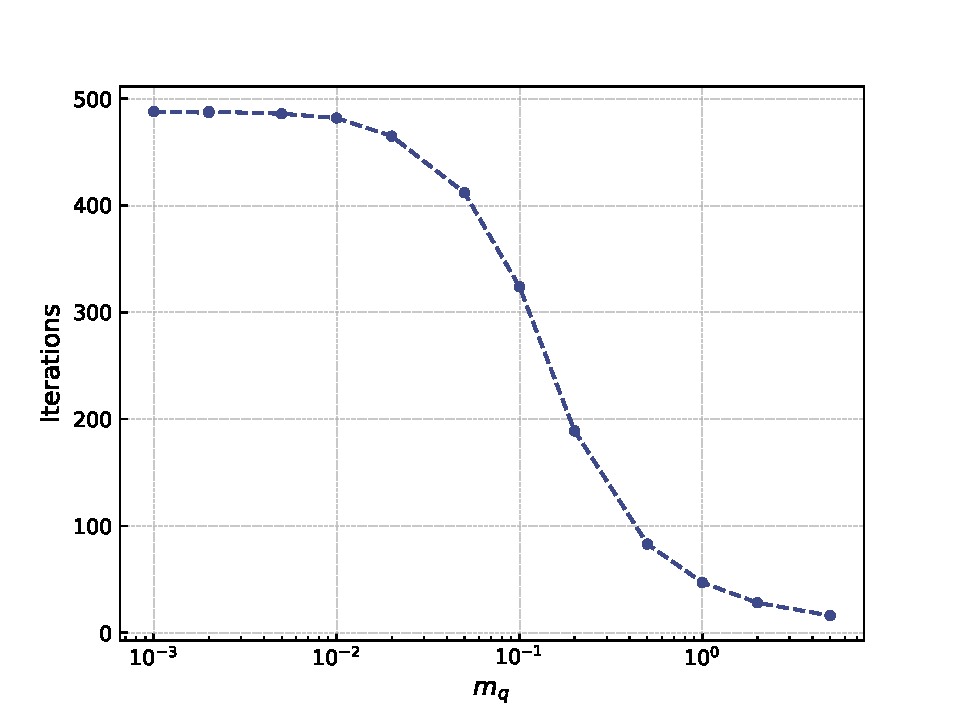
\includegraphics[scale=0.6]{figures/correlator/CGiter.pdf}
    \caption{CG iterations}
    \label{fig:correlator_CGiter}
\end{figure}
Figure \ref{fig:correlator_mass} reports the fermionic correlator as a function of $m_q$. One can see that a big bare quark mass results in a quick decay, while a small mass tends to deform the characteristic shape of the correlator. \\
Figure \ref{fig:correlator_CGiter} shows the number of iterations needed for convergence. While the exact number depends on the desired tolerance, one can clearly see that the number of iterations grows as $m_q \to 0$ due to an increase in the condition number \cite{cond_num_ref}. \textcolor{red}{does the condition number increase even more for naive fermions?} \\
We then choose three values of the bare quark mass and perform a fit according to \eqref{eq:correlator_mass_extraction}, in order to extract the physical mass and we compare it to the theoretical value given by \textcolor{red}{add ref. eq.}. The results are reported in figures \ref{fig:corr_small,fig:corr_medium,fig_corr_big} and table \ref{tab:mass_extraction_free}. \\~\\
\begin{table}
    \centering
    \begin{tabular}[pos]{cccc}
        \toprule 
        $m_q$ & teo & fit & err \\
        \midrule 
        1.0 & 0 & 0.6931537171644739 & 4e-20 \\
        0.1 & 0 & 0.09531020915059212 & 0.004 \\
        0.01 & 0 & 0.009950277657505842 & 0.8 \\
        \bottomrule
    \end{tabular}
\end{table}
\begin{figure}
    \centering
    \begin{subfigure}[b]{0.45\textwidth}
        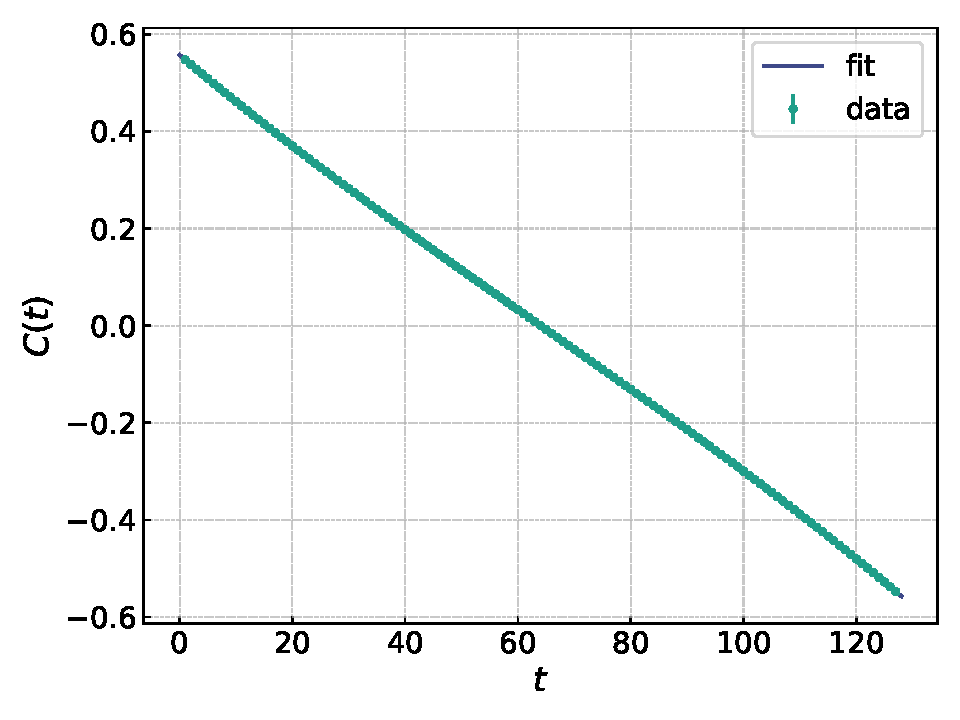
\includegraphics[width=\textwidth]{figures/correlator/corrs_free/corr_small.pdf}
        \caption{Caption for Image 1}
    \end{subfigure}
    \hfill
    \begin{subfigure}[b]{0.45\textwidth}
        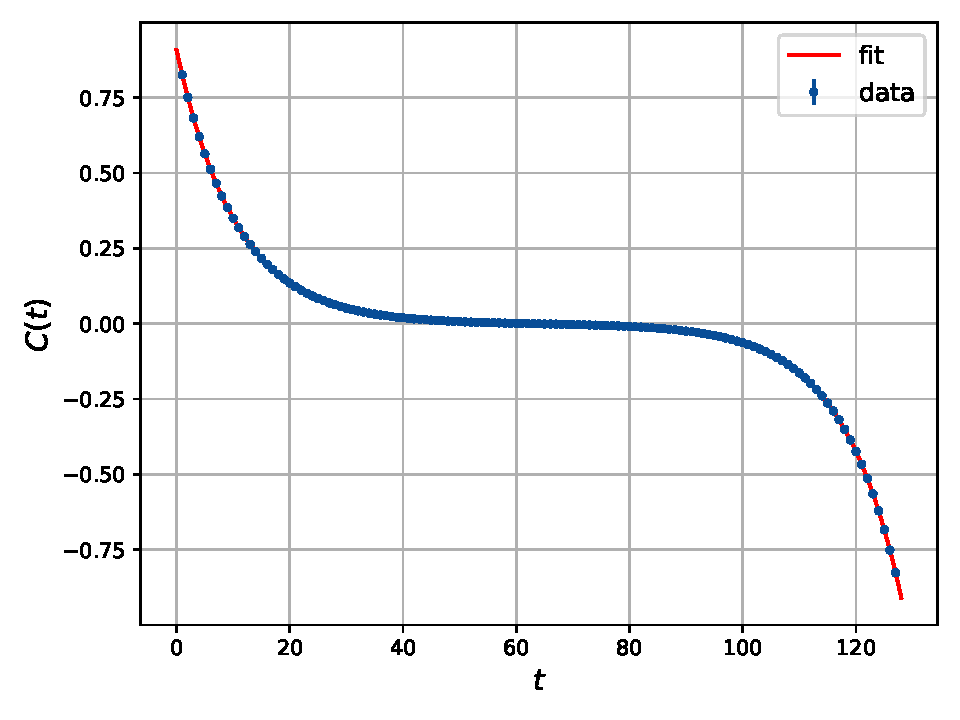
\includegraphics[width=\textwidth]{figures/correlator/corrs_free/corr_medium.pdf}
        \caption{Caption for Image 2}
    \end{subfigure}
    \\
    \vspace{20pt}
    \begin{subfigure}[b]{0.45\textwidth}
        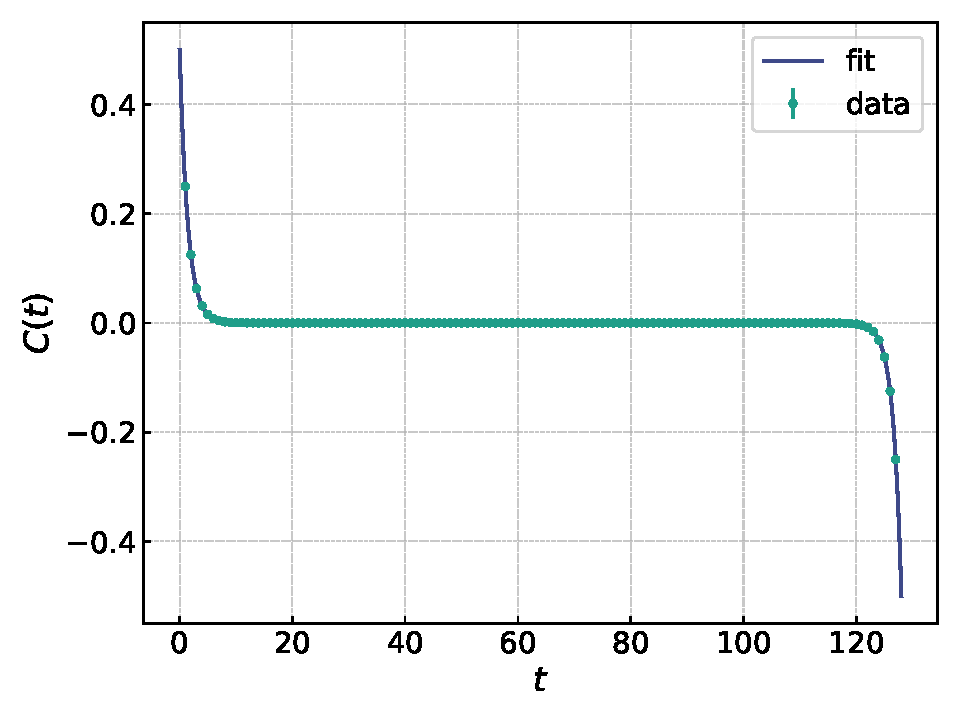
\includegraphics[width=\textwidth]{figures/correlator/corrs_free/corr_big.pdf}
        \caption{Caption for Image 3}
    \end{subfigure}
    \caption{Overall Caption for the Figure}
\end{figure}
The presence of a background field has the same effects on the correlator as a bare quark mass. In fact, if $\phi(x) = v$, one can simply redefine the bare mass as $M_q = m_q + g \, v$ and the properties of the fermionic correlator remain unchanged.

\newpage
\section{Classical-to-quantum interpolation}
\label{sec:classical_to_quantum}

\begin{figure}
    \centering
    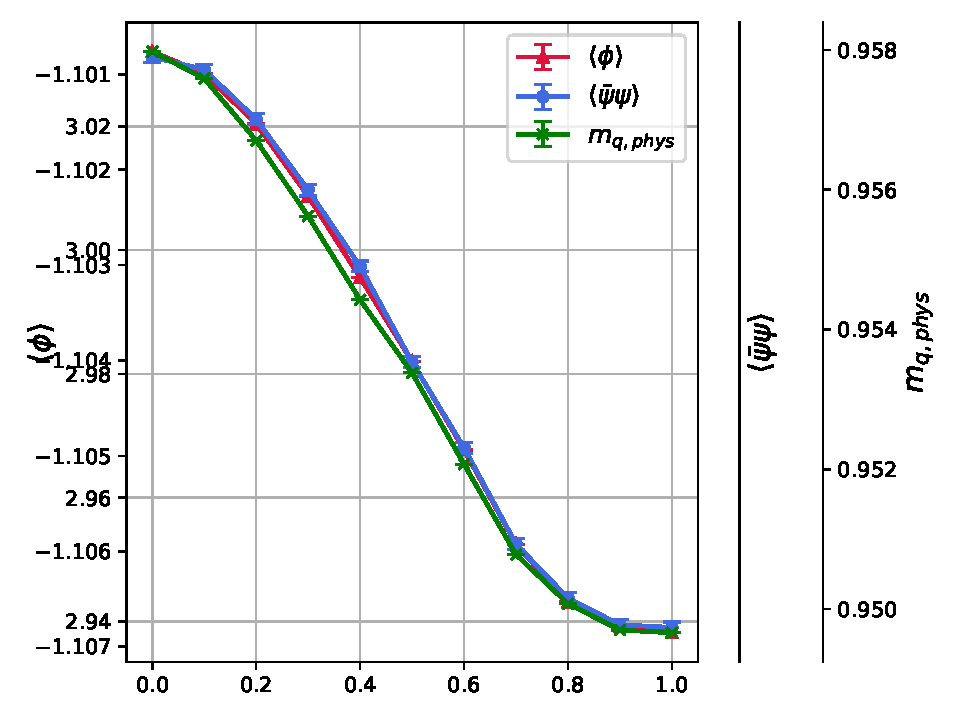
\includegraphics[scale=0.7]{figures/slide_broken/mag_cond.pdf}
\end{figure}

\begin{figure}
    \centering
    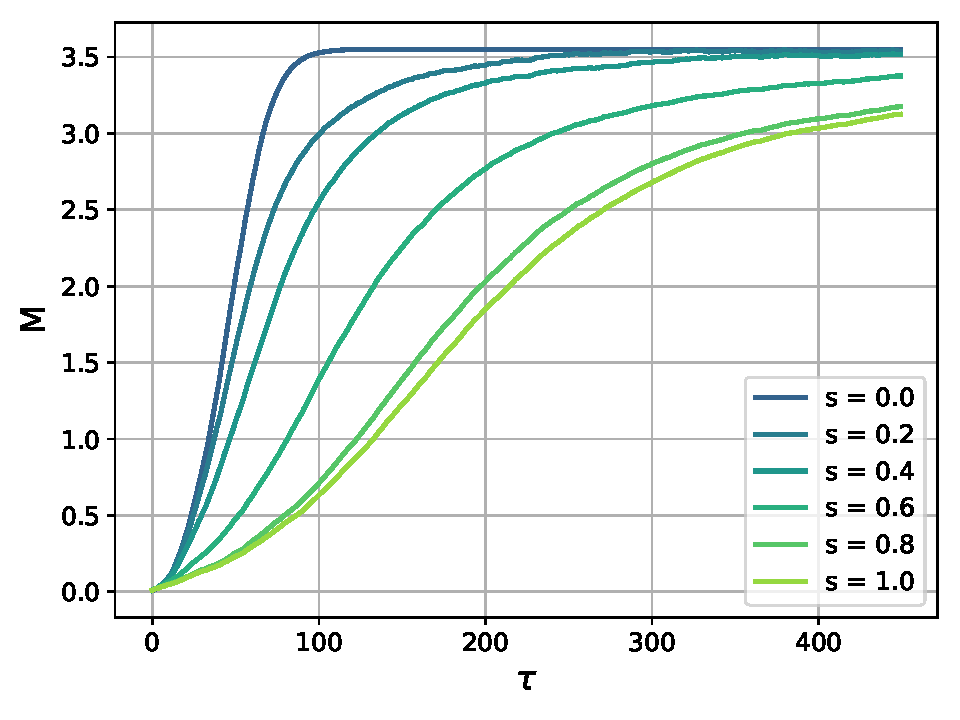
\includegraphics[width=0.5\textwidth]{figures/thermalisation_broken.pdf}
    \caption{}
    \label{fig:thermalisation_different_noise_fracs}
\end{figure}

Let us start by analising the coloured noise field in the simulation and relevant properties that emerge from it. We consider the Yukawa model described by the continuum action \eqref{eq:full_action_continuum} and its discrete vesion \eqref{eq:discretised_action}, \eqref{eq:discretised_effective_action}. \\~\\
Figure \ref{fig:thermalisation_different_noise_fracs} reports the Langevin evolution of the system for different noise fractions. The red line corresponds to the case $s=0$, namely a classical simulation, while the blue line corresponds to the case $s=1$, namely the fully quantum case. 
Note that a lower noise fraction is correlated to a faster convergence towards equilibrium. Moreover, low-distance fluctuations are suppressed due to the removal of the ultraviolet modes in the noise term. \\~\\
We now move on to analyse equilibrium properties. Coloured noise allows for a smooth interpolation between the fully quantum and fully classical picture, with a consequent shift of the expectation values of the observables. Figures \ref{fig:cheneso},\ref{fig:cheneso2} report, respectively, the magnetisation and the chiral condensate as a function of the noise fraction $s$. All the quntities in the classical action, including the coupling constants, are kept fixed while changing $s$.
Each figure reports two plots corresponding to two different parameter configurations. The COLOR1 line corresponds to a system in the symmetric phase, while the COLOR2 line correspond to the broken phase. The exact parameters for the two configurations are reported under the figure.
\textcolor{red}{non si puo parlare di fase rotta e simmetrica. inoltre commenta sulla relazione phi, psibarpsi con lambda=0}.

\newpage

\section{Cooling with coloured noise}


\begin{figure}
    \centering
    \begin{subfigure}[b]{0.45\textwidth}
        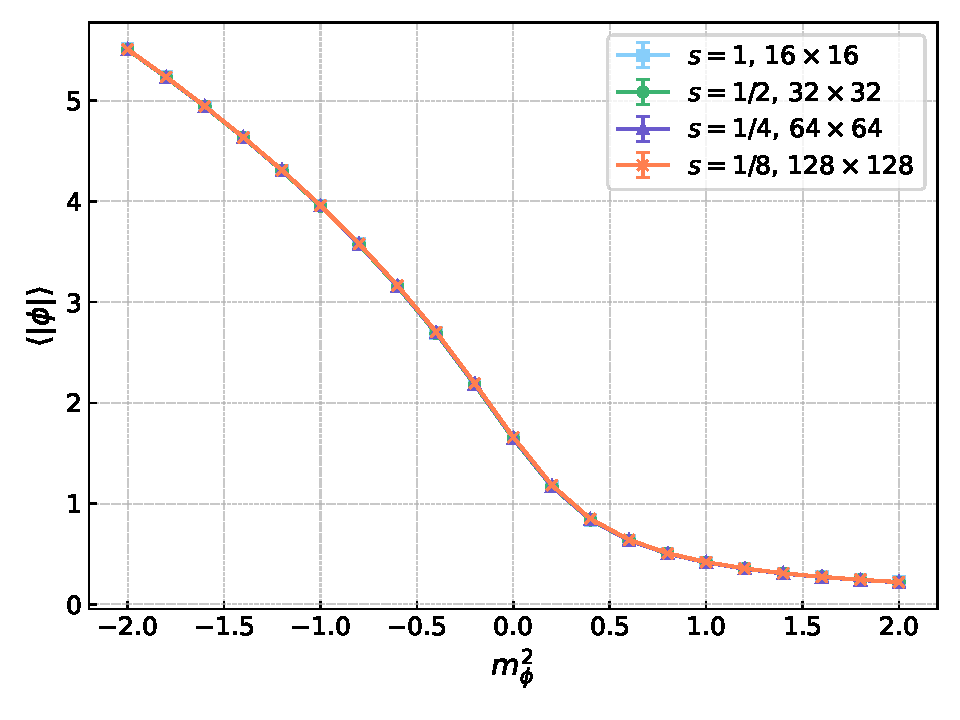
\includegraphics[width=\textwidth]{figures/cooling/mass_scan/magnetisation.pdf}
        \caption{Caption for Image 1}
    \end{subfigure}
    \hfill
    \begin{subfigure}[b]{0.45\textwidth}
        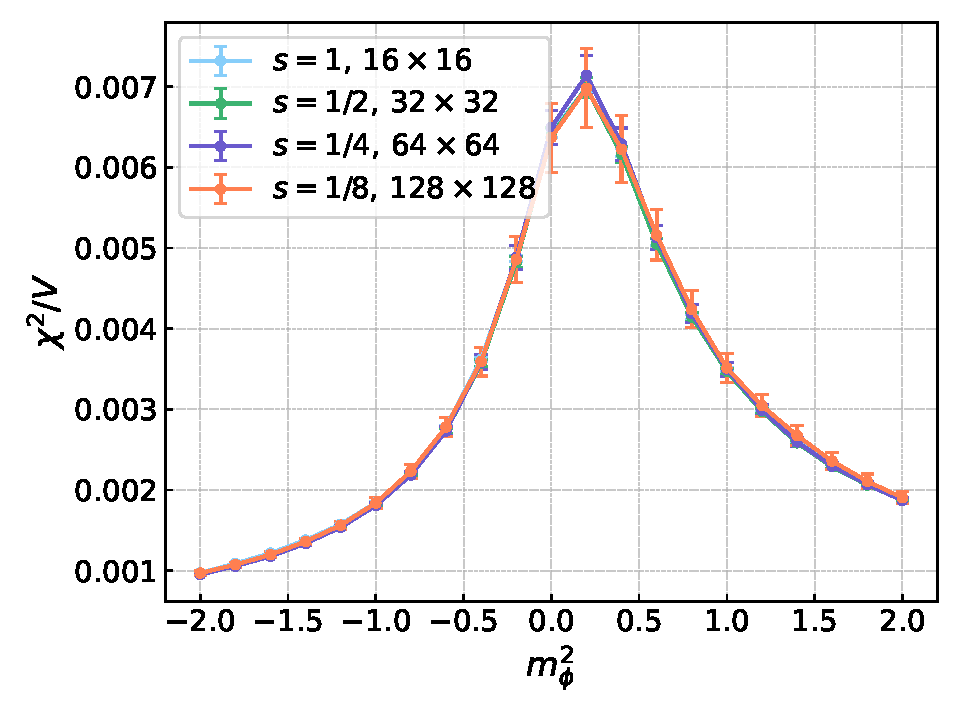
\includegraphics[width=\textwidth]{figures/cooling/mass_scan/susceptibility.pdf}
        \caption{Caption for Image 2}
    \end{subfigure}
    \\
    \vspace{10pt}
    \begin{subfigure}[b]{0.45\textwidth}
        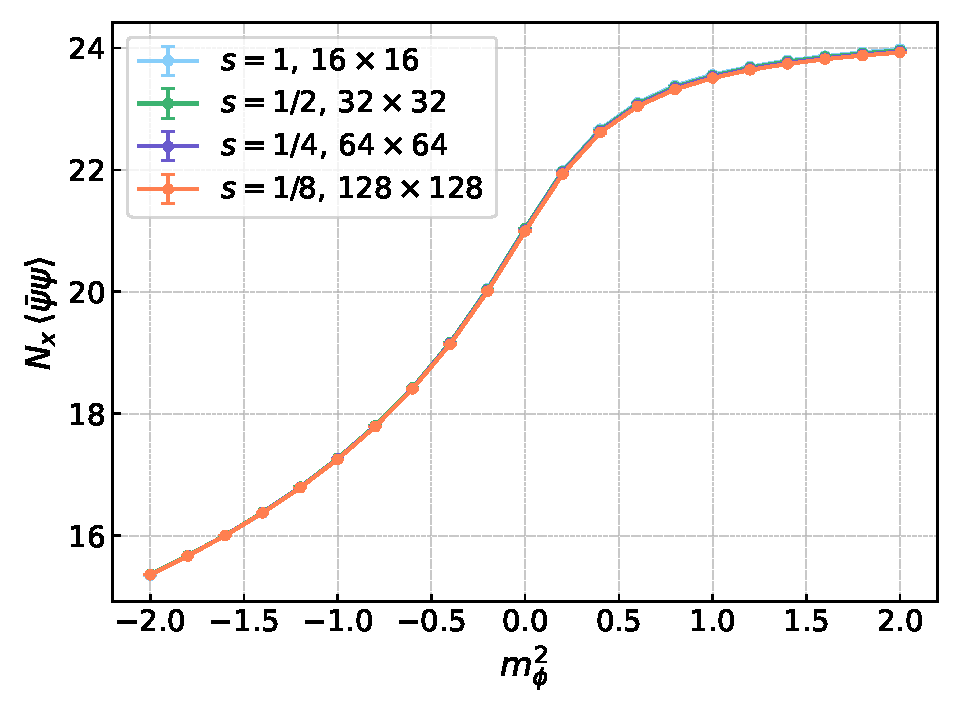
\includegraphics[width=\textwidth]{figures/cooling/mass_scan/condensate.pdf}
        \caption{Caption for Image 3}
    \end{subfigure}
    \caption{Overall Caption for the Figure}
\end{figure}

\begin{figure}
    \centering
    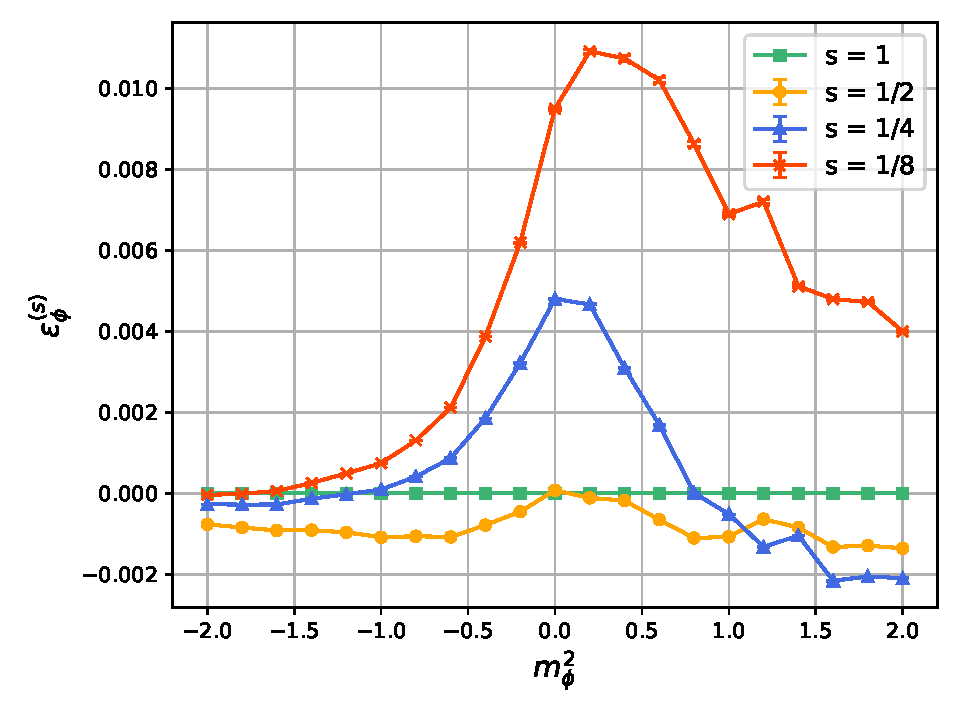
\includegraphics[scale=0.45]{figures/cooling/mass_scan/deviation.pdf}
    \label{fig:cooling}
\end{figure}

\begin{figure}
    \begin{minipage}{0.45\textwidth}
        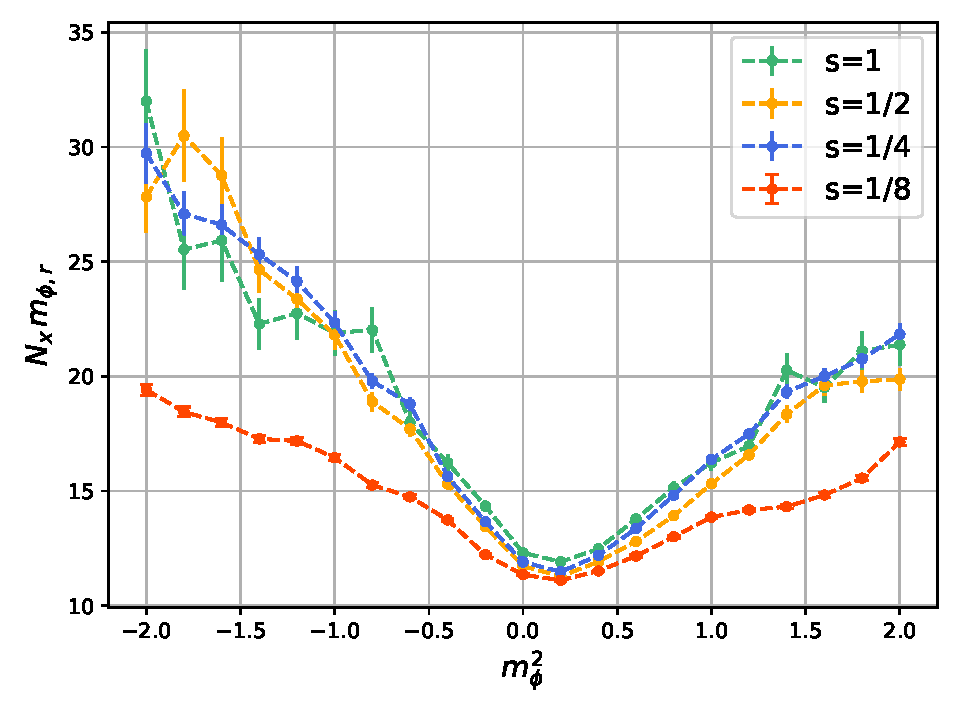
\includegraphics[scale=0.45]{figures/cooling/mass_scan/mphir.pdf}
    \end{minipage}
    \hfill 
    \begin{minipage}{0.45\textwidth}
        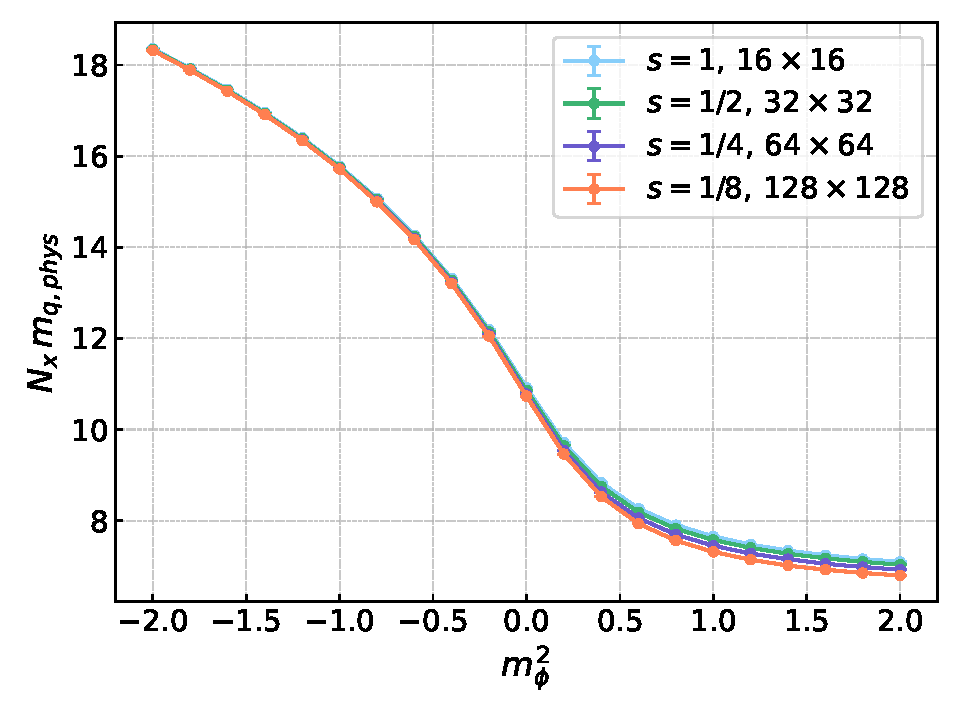
\includegraphics[scale=0.45]{figures/cooling/mass_scan/mqphys.pdf}
    \end{minipage}
\end{figure}


\newpage



\newpage
\section{Chiral fermions and a glimpse on the chiral phase transition}
\label{sec:chiral_PT}

\begin{figure}
    \centering
    \begin{minipage}{0.45\textwidth}
        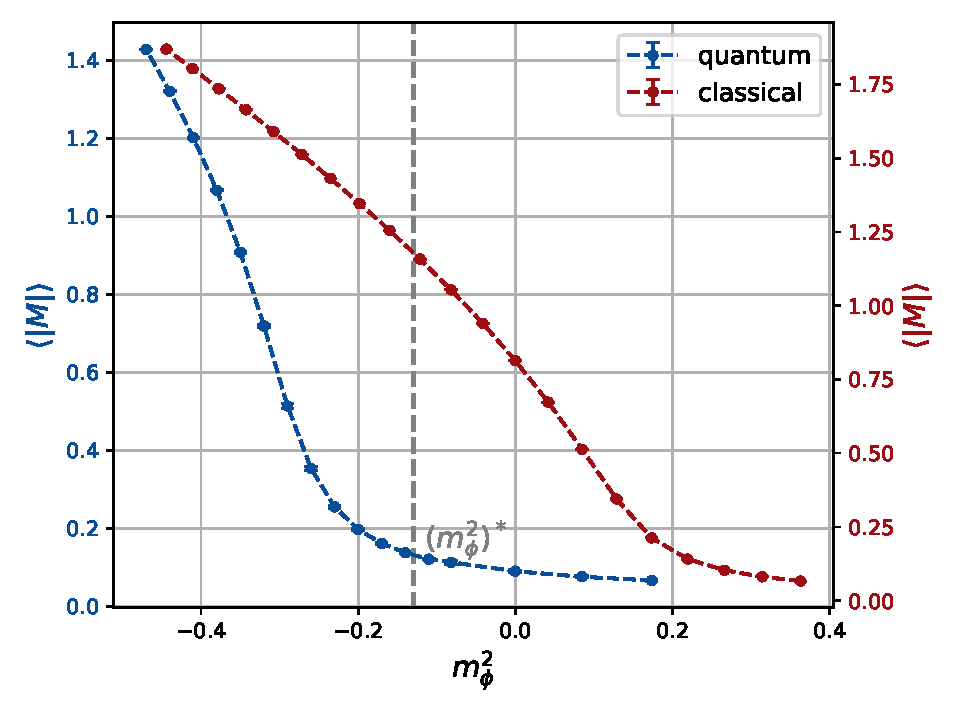
\includegraphics[scale=0.5]{figures/chiral_PT/mass_scan/magnetisation.pdf}
    \end{minipage}
    \hfill
    \begin{minipage}{0.45\textwidth}
        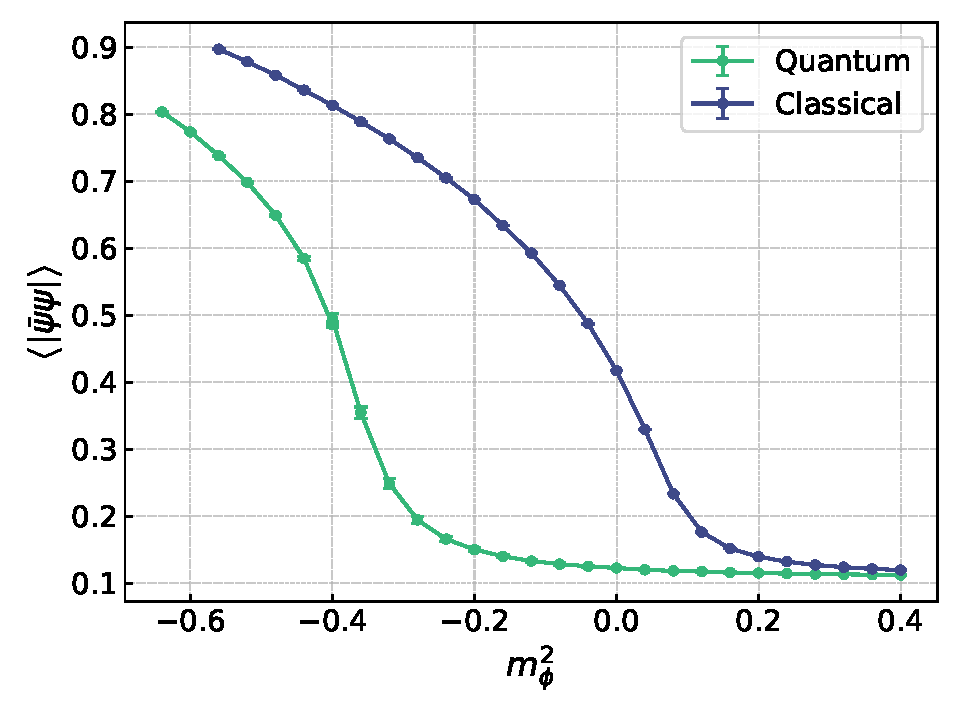
\includegraphics[scale=0.5]{figures/chiral_PT/mass_scan/condensate.pdf}
    \end{minipage}
    \begin{minipage}{0.45\textwidth}
        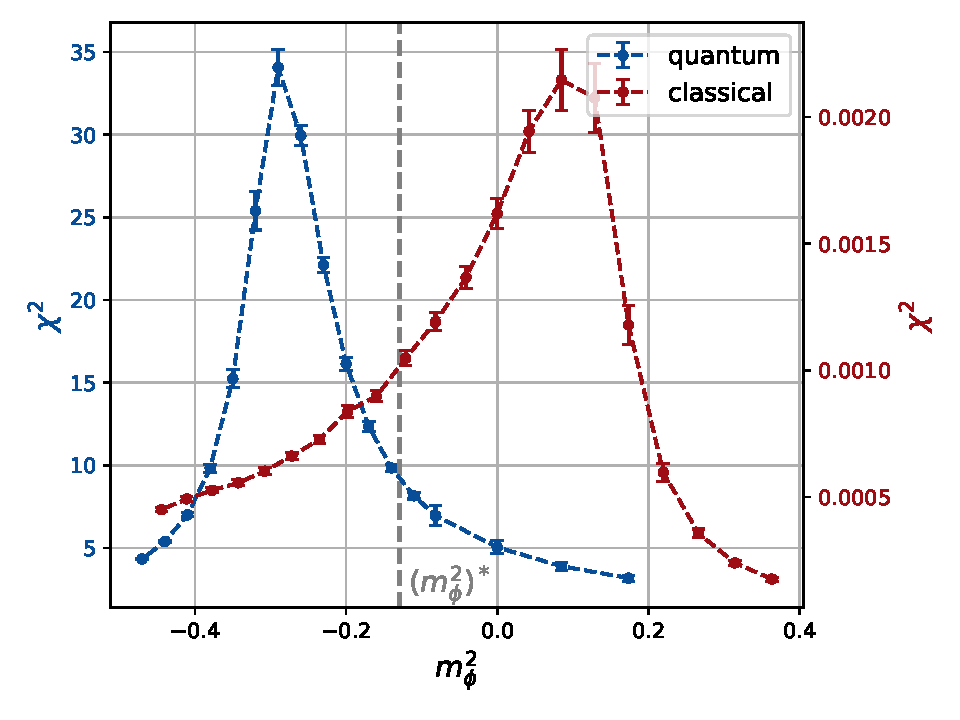
\includegraphics[scale=0.5]{figures/chiral_PT/mass_scan/susceptibility.pdf}
    \end{minipage}
\end{figure}

As explained in section \ref{sec:yukawa}, in the continuum theory chiral symmetry can be broken either explicitly via a finite bare quark mass, or spontaneously if the field gains a non-zero expectation value. Moreoveor, in the discrete formulation, the introduction of the Wilson term also contributes to the explicit breaking of chiral symmetry \textcolor{red}{add reference}, as explained in section \ref{sec:discrete}. This, in particular, means that chiral symmetry is explicitly broken also for $m_q \to 0$. Because of this, one needs a new definition for bare mass $M_q$, which takes into account the Wilson term contribution, such that chiral symmetry is restored in the limit $M_q \to 0$ for vanishing expectation value of the field $\phi$. A convenient way to define such $M_q$ is the following. SSB chiral symmetry $\to$ 3 goldstone massless bosons, the pions. If the bare quark mass is zero, the physical mass of the pions has to be zero. Hence one can extract this mass on the lattice and tune $m_q$ such that this is zero. While this is the correct way to proceed, it is very time takin since one must do mass scans and extrapolations close to singular Dirac operator. This is not the way we pursue here. Instead here we just consider naive fermions and take the limit $m_q \to 0$. This represents a physical theory with $2N_f = 4$ degenerate quarks. This is just done for the purpose of showing some interest properties of coloured noise and not (yet) to match any physical result. \\~\\
In figure \ref{fig:chiral_symmetry_breaking} some observables are reported as a function of the noise fraction $s$ for different values of the bare quark mass. In the classical theory ($s=0$) the order parameters $\left\langle|\phi|\right\rangle, \left\langle\bar\psi \psi\right\rangle$ are, in absolute value, bigger than in the quantum case ($s=1$).  As the chiral limit is approached $m_q \to 0$, the figure shows that the classical system lies in the broken phase, while in the quantum settings the symmetry is restored. \textcolor{red}{Discuss general phase structure looking at both $\phi$ and $\bar\psi\psi$}. One can see that as $m_q$ is reduced, the systems shifts from a crossover to a second order phase transition, ahighligthed by the susceptibility $\chi^2$ and the binder parameter $U_L$.

\textcolor{red}{This would be better discussed as a function of bare scalar mass:} \\
The difference gets more sharped as the base mass decreases, since the theory is closer to the chiral limit discussed above, which corresponds to the case $m_q=0$. In this limit the systems goes under a second phase transition, highlighted by a peak in the susceptibility and and abrubt change in the Binder cumulant. In contrast, for finite mass,  there is smooth crossover where the order parameters change continuously.

\begin{figure}[h]
\centering
\begin{minipage}{0.45\textwidth}	
	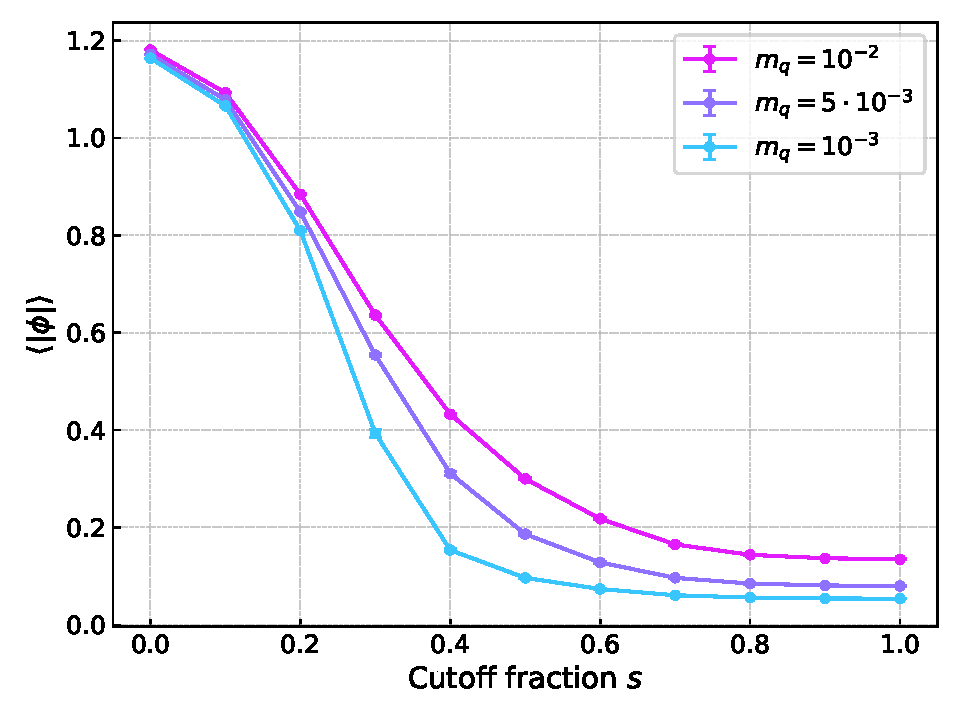
\includegraphics[scale=0.48]{figures/chiral_PT/magnetisation.pdf}
\end{minipage}
\hfill
\begin{minipage}{0.45\textwidth}	
	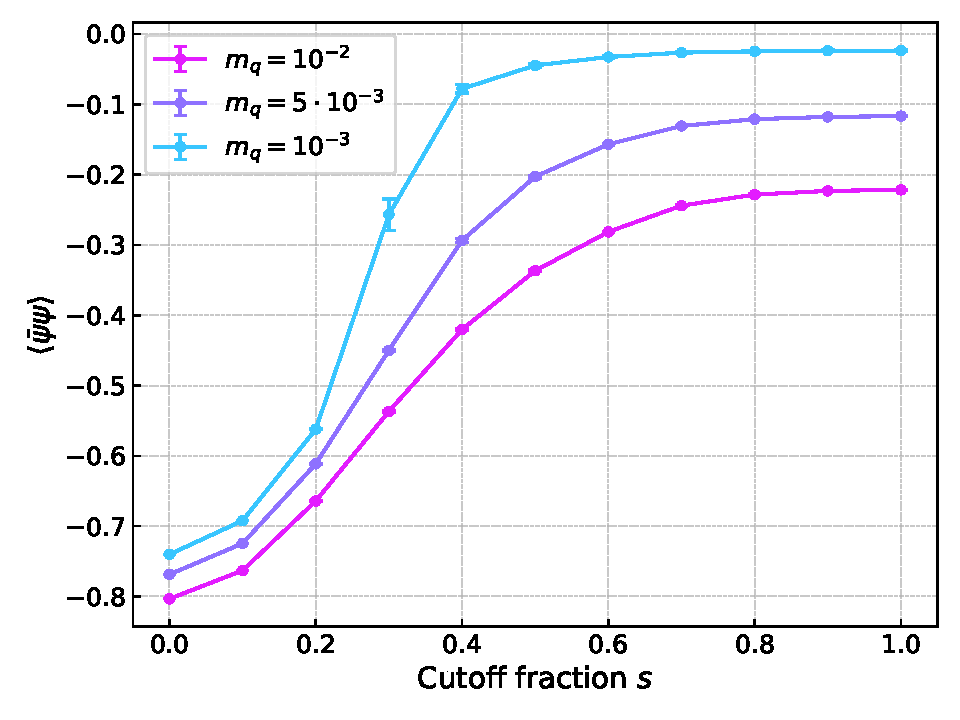
\includegraphics[scale=0.48]{figures/chiral_PT/condensate.pdf}
\end{minipage}
\begin{minipage}{0.45\textwidth}	
	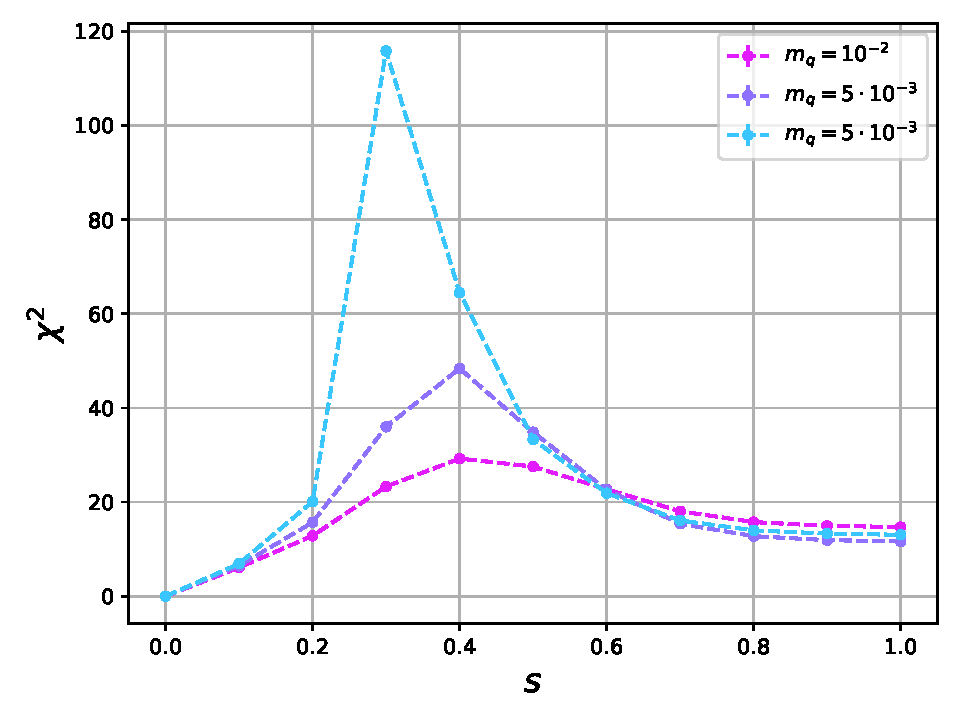
\includegraphics[scale=0.48]{figures/chiral_PT/susceptibility.pdf}
\end{minipage}
\hfill
\begin{minipage}{0.45\textwidth}
	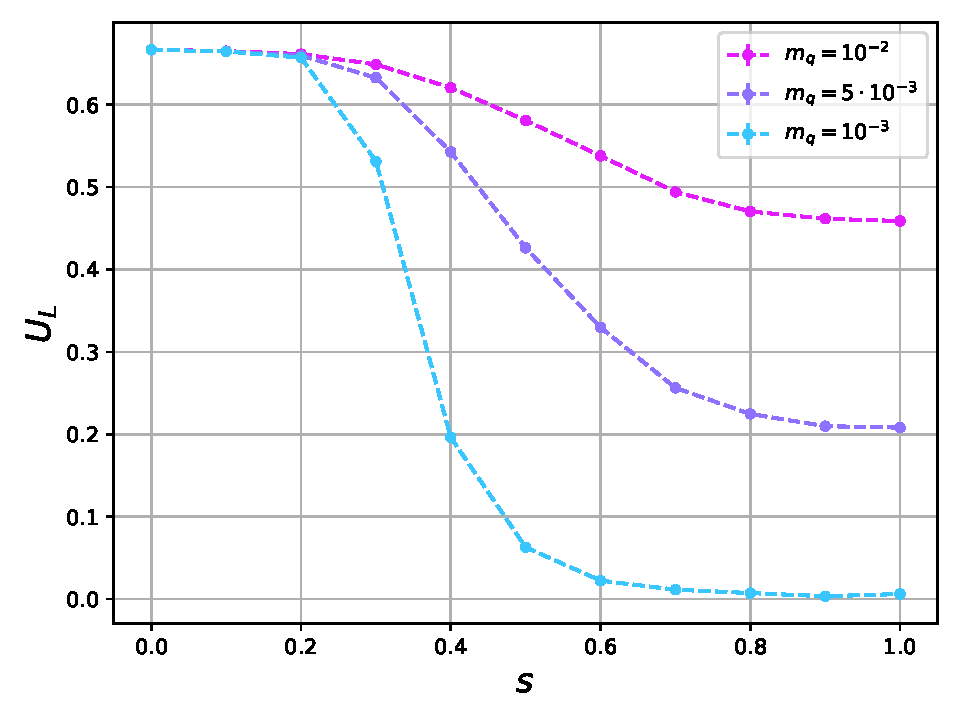
\includegraphics[scale=0.48]{figures/chiral_PT/binder.pdf}
\end{minipage}
\hfill
\caption{Chiral symmetry breaking}
\label{fig:chiral:symmetry_breaking}
\end{figure}


